\section{Transformations}

\begin{definition}
    A \emph{projective mapping} between a projective plane $\mathbb{P}^2$ and another projective plane $\mathbb{P}^{'2}$ is an invertible mapping which preserves co-linearity:
    \[h:\mathbb{P}^2 \rightarrow \mathbb{P}^{'2}, x^{'}=h(x),x_1,x_2,x_3 \textnormal{ are colinear}\]
    \[\Leftrightarrow\]
    \[x_1^{'}=h(x_1),x_2^{'}=h(x_2),x_3^{'}=h(x_3) \textnormal{ are colinear}\]
\end{definition}
Projective mapping is also called projectivity or homography. 
\begin{example}
    Mappings between two planes induced by central projection are projective, since they preserve co-linearity. 
    \begin{figure}[H]
        \centering
        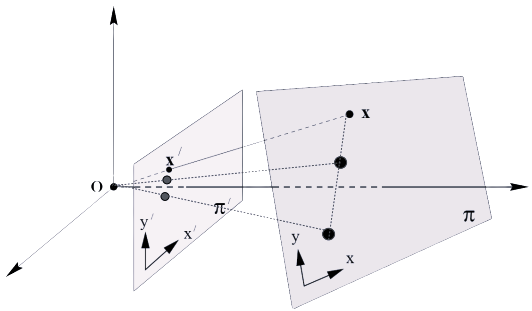
\includegraphics[width=0.4\linewidth]{images/map1.png}
    \end{figure}
    Mapping between a planar scene and its image is a homography, since it is induced by a central projection
    \begin{figure}[H]
        \centering
        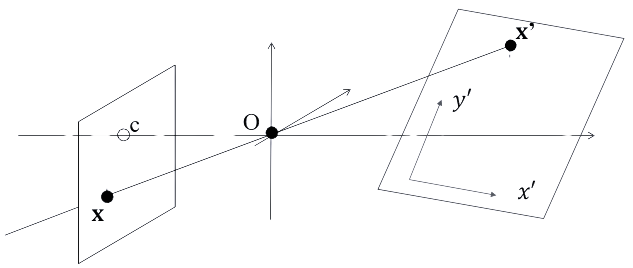
\includegraphics[width=0.4\linewidth]{images/map2.png}
    \end{figure}
    Mapping between two images of a planar scene is a homography.
    \begin{figure}[H]
        \centering
        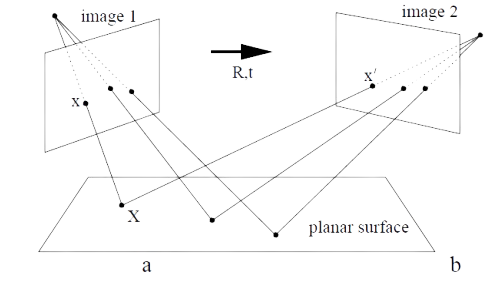
\includegraphics[width=0.4\linewidth]{images/map3.png}
    \end{figure}
    Two images of a 3D scene, taken by a camera rotating around its center are related by a homography, since the second image is a central projection of the first image. 
    \begin{figure}[H]
        \centering
        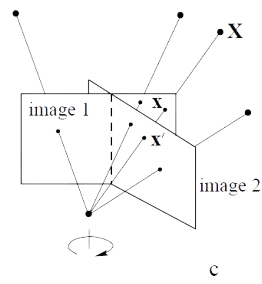
\includegraphics[width=0.3\linewidth]{images/map4.png}
    \end{figure}
    The shadow cast by a planar silhouette onto a ground plane is a projective transformation of the planar silhouette, since they are related by a central projection. 
    \begin{figure}[H]
        \centering
        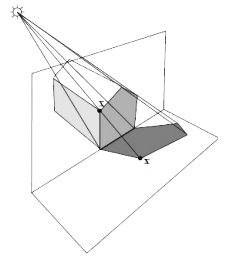
\includegraphics[width=0.3\linewidth]{images/map5.png}
    \end{figure}
\end{example}
\begin{theorem}
    A mapping $h:\mathbb{P}^{2} \rightarrow \mathbb{P}^{'2}$ is projective if and only if there exists an invertible $3 \times 3$ matrix $H$ such that for any point in $\mathbb{P}^{2}$ represented by the vector $x$, is $h(x)=Hx$, where: 
    \[H=\begin{bmatrix}
        h_{11} & h_{12} & h{13} \\
        h_{21} & h_{22} & h{23} \\
        h_{31} & h_{32} & h{33} 
    \end{bmatrix}\]
\end{theorem}
Projective mappings are linear when expressed in homogeneous coordinates, but they do not exhibit linearity when represented in Cartesian coordinates.

According to the theorem, if we have $h(x)=x^{'}=Hx$, then multiplying the matrix $H$ by any nonzero scalar $\lambda$ still satisfies the relation for the same points, giving us $x^{'}=\lambda Hx$. 
Therefore, any nonzero scalar multiple of the matrix $H$ represents the same projective mapping as $H$.
As a result, we can conclude that $H$ is a homogeneous matrix.
Despite having nine entries, it possesses only eight degrees of freedom, specifically the ratios between its elements. 
Consequently, we can estimate $H$ using just four point correspondences.
Each point correspondence, expressed as $x^{'}=Hx$, provides two independent equations in this estimation process.
\newpage
\begin{definition}
    A \emph{homography} transforms various geometric entities as follows:
    \begin{enumerate}
        \item It maps a point $x$ to a point $x^{'}$, where the transformation is expressed as: 
            \[x \rightarrow H x=x^{'}\]
        \item It maps a line $l$ to a line $l^{'}$, and this transformation is represented as: 
            \[l \rightarrow H^{-T} l=l^{'}\]
        \item It maps a conic $C$ to a conic $C^{'}$, and the transformation is given by: 
            \[C \rightarrow H^{-T} CH^{-1}=C^{'}\]
        \item It maps a dual conic $C^{*}$ to a dual conic $C^{*'}$, with the transformation being: 
            \[C^{*} \rightarrow H C^{*}H^{T}=C^{*'}\]
    \end{enumerate}
\end{definition}
\begin{proof}[of mapping two]
    To transform the equation of the line in terms of $x$, given by $l^Tx=0$, into a constraint on $x^{'}=Hx$, we combine the two equations, resulting in a linear equation on $x^{'}$: 
    \[l^{'T}x^{'}=0\]
    Here, $l^{'T}=l^{T}H^{-1}$. 
    Thus, we have:
    \[l^{'}=H^{-T}l\]
\end{proof}
\begin{proof}[of mapping three]
    To transform the equation of the conic in terms of $x$, given by $x^{T}Cx=0$, into a constraint on $x^{'}=Hx$, we have$x=H^{-1}x^{'}$ and $x^{T}=x^{iT}H^{-T}$. 
    Combining these three equations, we obtain a linear equation on $x^{'}$: 
    \[x^{'T}C^{'}x^{'}=0\]
    Hence, we have:
    \[C^{'}=H^{-T} CH^{-1}\]
\end{proof}
\begin{proof}[of mapping four]
    or the transformation of a dual conic, we apply the same idea, yielding:
    \[C^{*'}=H C^{*}H^{T}\]
\end{proof}
The point-line incidence is preserved. 
\begin{proof}
    Let $x$ be a point on the line $l$. 
    This is expressed as $l^Tx=0$. 
    When we apply the projective transformation $H$ to both $x$and $l$, resulting in $Hx=x^{'}$ and $H^{-1}l=l^{'}$, they remain incident if $l^{'T}x^{'}=0$:
    \[l^{'T}x^{'}=l^{T}H^{-1}x^{'}=l^{T}H^{-1}Hx=l^{T}x=0\]
\end{proof}

\subsection{Vanishing points and vanishing line}
The point that is common to both parallel lines $l_1={\begin{bmatrix} a & b & c_1 \end{bmatrix}}^{T}$ and $l_2={\begin{bmatrix} a & b & c_2 \end{bmatrix}}^{T}$ is the point $x={\begin{bmatrix} b & -a & 0 \end{bmatrix}}^{T}$. 
This point is situated at infinity along the direction of both lines.
When seeking the common point of the infinite lines $l_i$, we find that they all share the same point:
\[x_{\infty}={\begin{bmatrix} b & -a & 0 \end{bmatrix}}^{T}\]
Hence, it becomes apparent that all these lines converge at ${\begin{bmatrix} b & -a & 0 \end{bmatrix}}^{T}$. 

If we apply a projective transformation to all the aforementioned parallel lines $l_i$, we obtain the transformed lines $l_i^{'}$. 
The common point $x_{\infty}$, shared by all lines $l_i$, is mapped to a point $x_{\infty}^{'}$ which belongs to each of the lines $l_i^{'}$. 
\begin{figure}[H]
    \centering
    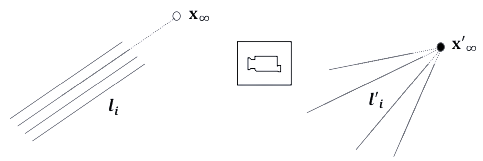
\includegraphics[width=0.5\linewidth]{images/vanishing.png}
\end{figure}
Therefore, we can assert that all lines $l_i^{'}$ intersect at the point $x_{\infty}^{'}=Hx_{\infty}$, referred to as the vanishing point associated with the direction $(b,-a)$ of the parallel lines. 
\begin{theorem}
    The image of a set of parallel lines $l_i$ is a set of lines $l_i^{'}$ concurrent at a common point $x^{'}$ known as the vanishing point of the direction of lines $l_i$. 
\end{theorem}

By applying a projective transformation to the line at infinity $l_{\infty}$, we obtain a line $l_{\infty}^{'}$. 
This line intersects the image all the points at the infinity $x_{\infty}$ from  the original plane. 
Consequently, the vanishing line $l_{\infty}^{'}$ can be determined from two vanishing points. 
\begin{figure}[H]
    \centering
    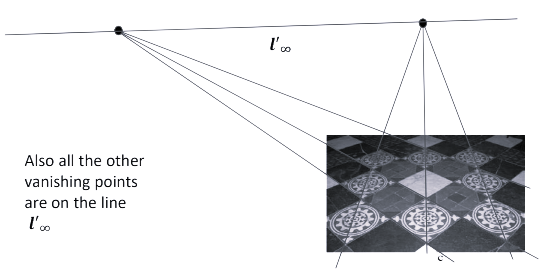
\includegraphics[width=0.5\linewidth]{images/vanishingline.png}
\end{figure}

\subsection{Polarity}
Polarity remains unaltered in the presence of projective mappings.
The polar line $l=Cx$ corresponding to a point $x$ with respect to a conic $C$ gets mapped to the polar line of the transformed point $x^{'} = Hx$ with respect to the transformed conic:
\[C^{'}=H^{-T}CH^{-1}\]
\begin{proof}
    This property holds because:
    \[C^{'}x^{'}=H^{-T}CH^{-1}Hx=H^{-T}Cx=H^{-T}l=l^{'}\]
    Therefore, the polar line of the transformed point aligns with the polar line of the original point.
\end{proof}
\begin{figure}[H]
    \centering
    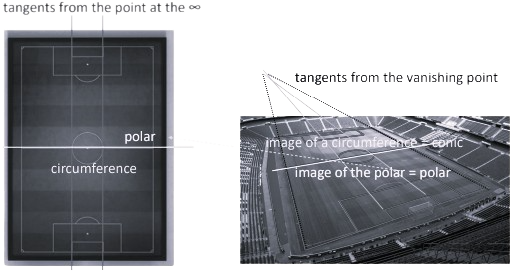
\includegraphics[width=0.75\linewidth]{images/polarity.png}
\end{figure}
In conclusion, as polarity remains intact under projective mappings, conjugacy is similarly preserved, and the relationship $CR=-1$ is also upheld.

\subsection{Cross ratio}
Given a line defined by four points with the following relationships:
\[x_1=\propto_1Y+\beta_1Z\]
\[x_2=\propto_2Y+\beta_2Z\]
The cross ratio is expressed as:
\[CR_{X_1,X_2,Y,Z}=\dfrac{\beta_1/\alpha_1}{\beta_2/\alpha_2}\]
Upon applying a projective transformation $H$ to these four points:
\[Y^{'}=HY \:\:\:\:\:\: Z^{'}=HZ\] 
\[x^{'}_1=HX_1=x_1=\propto_1Y^{'}+\beta_1Z^{'} \:\:\:\:\:\: x^{'}_2=HX_2=\propto_2Y^{'}+\beta_2Z^{'}\]
The coefficients of the linear combination remain the same. 
Hence, the cross ratio is conserved, maintaining its original value:
\[CR_{X_1^{'},X_2^{'},Y^{'},Z^{'}}=\dfrac{\beta_1/\alpha_1}{\beta_2/\alpha_2}=CR_{X_1,X_2,Y,Z}\]

\subsection{Isometries}
Isometries possess three degrees of freedom, which include translation denoted as $t$ and the rotation angle represented by $\vartheta$. 
Consequently, the invariants of this transformation encompass lengths, distances, and areas.
\begin{figure}[H]
    \centering
    
\includegraphics[width=0.25\linewidth]{images/isometry.png}
\end{figure}
\begin{definition}
    The \emph{orthogonal matrix} $R_{\perp}$ is defined as follows: 
    \[R_{\perp}^{-1}=R_{\perp}^{T}\]
\end{definition}
Hence, the matrix $H_I$ for isometries takes the following form:
\[H_I=
\begin{bmatrix}
    \cos \vartheta & -\sin \vartheta & t_x \\
    \sin \vartheta & \cos \vartheta & t_y \\
    0 & 0 & 1
\end{bmatrix}\]
Here, $
\begin{bmatrix}
    \cos \vartheta & -\sin \vartheta \\
    \sin \vartheta & \cos \vartheta
\end{bmatrix}
=R_{\perp}$
\begin{figure}[H]
    \centering
    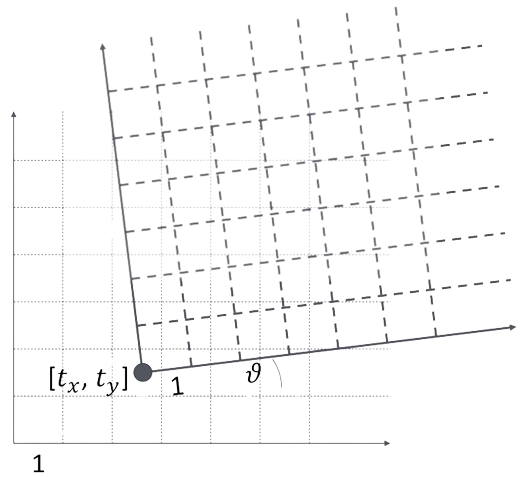
\includegraphics[width=0.25\linewidth]{images/isometry1.png}
    \caption{Isometry}
\end{figure}

\subsection{Similarities}
Similarities are characterized by four degrees of freedom, encompassing the translation, denoted as $t$; the scale, represented by $s$; and the rotation angle, expressed as $\vartheta$.
Consequently, the invariants of this transformation encompass the ratio of lengths and angles.
Furthermore, the circular points $I$ and $J$ remain invariant throughout this transformation.
\begin{figure}[H]
    \centering
    
\includegraphics[width=0.2\linewidth]{images/similarity.png}
\end{figure}
Hence, the matrix $H_S$ for similarities is as follows:
\[H_I=
\begin{bmatrix}
    s\cos \vartheta & -s\sin \vartheta & t_x \\
    s\sin \vartheta & s\cos \vartheta & t_y \\
    0 & 0 & 1
\end{bmatrix}\]
Here, $
\begin{bmatrix}
    s\cos \vartheta & -s\sin \vartheta \\
    s\sin \vartheta & s\cos \vartheta
\end{bmatrix}
=sR_{\perp}$
\begin{figure}[H]
    \centering
    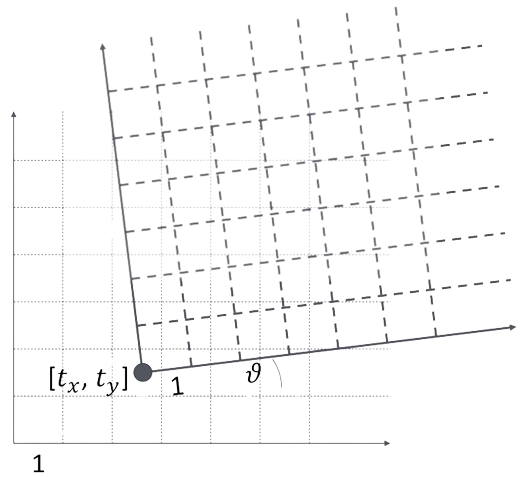
\includegraphics[width=0.25\linewidth]{images/isometry1.png}
    \caption{Similarity}
\end{figure}

\subsection{Affinities}
Affinities exhibit six degrees of freedom, consisting of the sub-matrix $A$ and the translation component. 
As a result, the invariants of this transformation encompass parallelism, the ratio of parallel lengths, and the ratio of areas. 
The matrix $A$ is defined as a $2 \times 2$ matrix with a rank of two. 
Additionally, the line at infinity, denoted as $l_{\infty}$, remains invariant throughout the transformation.
\begin{figure}[H]
    \centering
    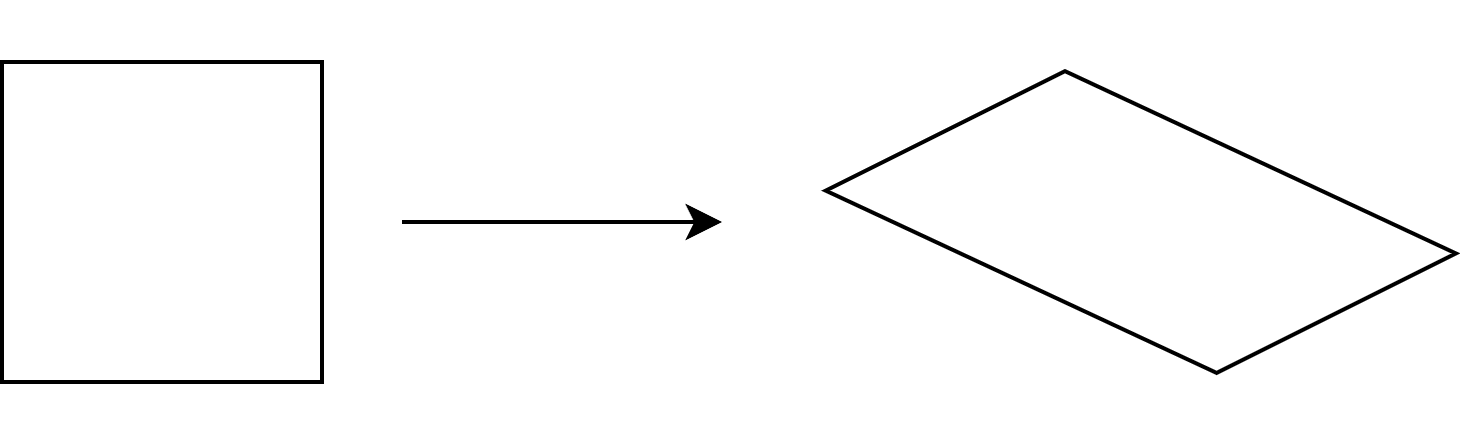
\includegraphics[width=0.25\linewidth]{images/affinities.png}
\end{figure}
Hence, the matrix $H_A$ for affinities takes the following form:
\[H_I=
\begin{bmatrix}
    a_{11} & a_{21} & t_x \\
    a_{12} & a_{21} & t_y \\
    0 & 0 & 1
\end{bmatrix}\]
Here, $
\begin{bmatrix}
    a_{11} & a_{21} \\
    a_{12} & a_{21} \\
\end{bmatrix}
=A$
\begin{figure}[H]
    \centering
    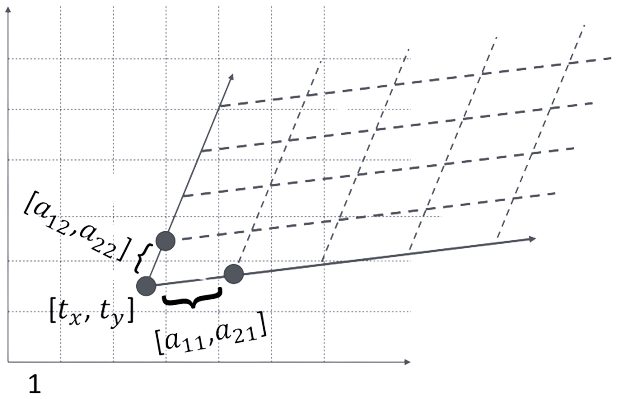
\includegraphics[width=0.3\linewidth]{images/affinities1.png}
\end{figure}

\subsection{Projectivities}
Projectivities possess eight degrees of freedom, encompassing the sub-matrix $A$, the vector $v$, and the translation component. 
Therefore, the invariants of this transformation include co-linearity, incidence, and the order of contact.
The matrix $A$ is defined as a $2 \times 2$ matrix with a rank of two. 
Furthermore, the cross ratio remains invariant throughout this transformation.
\begin{figure}[H]
    \centering
    
\includegraphics[width=0.25\linewidth]{images/projectivities.png}
\end{figure}
Hence, the matrix $H_P$ for projectivities takes the following form:
\[H_I=
\begin{bmatrix}
    a_{11} & a_{21} & t_x \\
    a_{12} & a_{21} & t_y \\
    v_1 & v_2 & 1
\end{bmatrix}\]
Here, $
\begin{bmatrix}
    a_{11} & a_{21} \\
    a_{12} & a_{21} \\
\end{bmatrix}
=A$
\begin{figure}[H]
    \centering
    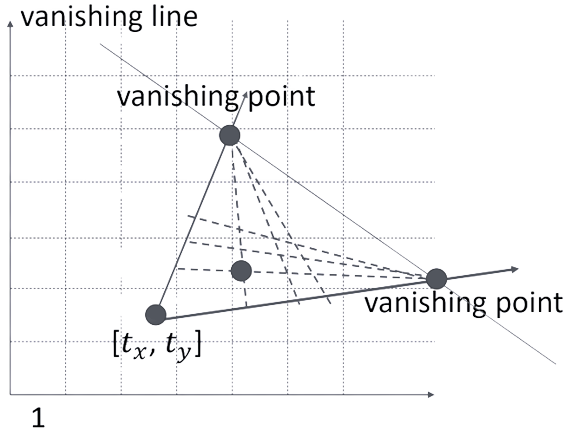
\includegraphics[width=0.25\linewidth]{images/projectivities1.png}
    \caption{Affinity}
\end{figure}